\documentclass{scrreprt}
\usepackage{lmodern}
\author{Andreas Schachner}
\title{Dokumentation zum Uni-Heidelberg-App-Projekt}
\usepackage[T1]{fontenc}
\usepackage[ngerman]{babel} 
\usepackage[automark,headsepline,plainheadsepline]{scrpage2}
\usepackage{endnotes}
\usepackage{csquotes}
\usepackage{hyperref}
\hypersetup{colorlinks=true,urlcolor=blue,linkcolor=blue}
\setcounter{tocdepth}{2}
\pagestyle{scrheadings}
\ihead[\rightmark]{\rightmark} \chead[\pagemark]{}
\usepackage{pst-all}
\usepackage{fontspec}
\newfontfamily{\codefont}{Menlo}

\usepackage{color,xcolor}
\definecolor{nsclass}{RGB}{124,32,176}
\definecolor{atnotation}{RGB}{204,0,164}
\definecolor{import}{RGB}{128,70,30}
\definecolor{comment}{RGB}{0,140,0}
\definecolor{string}{RGB}{229,0,0}
\definecolor{method}{RGB}{70,0,134}
\definecolor{class}{RGB}{59,131,138}
\definecolor{custommethod}{RGB}{32,90,95}
\definecolor{number}{RGB}{56,0,225}
\definecolor{customgray}{RGB}{211,211,211}
\definecolor{highlight}{RGB}{255,243,153}

\usepackage{listings}
\lstloadlanguages{[Objective]C,bash}
\lstset{language=[Objective]C,tabsize=4, keepspaces=false,
    xleftmargin=0em,xrightmargin=-1em, aboveskip=1em, % Margin adjustment
    %backgroundcolor=\color{customgray},    % Background color (Default:gray)
    frame=none,                            % Frame not needed
    breakindent=22pt,
    numbers=left,stepnumber=1,numberstyle=\tiny\color{black}\codefont,
    basicstyle=\fontsize{9pt}{1em}\selectfont\codefont,
    commentstyle=\fontsize{9pt}{0.75em}\selectfont\codefont\color{comment},
    showspaces=false,
    showstringspaces=false,
    flexiblecolumns=true,
    breaklines=true, breakautoindent=true,breakindent=4em,
    escapeinside={/*@}{@*/},
    morecomment=[s][\color{string}]{@"}{"},
    morecomment=[l][\color{import}]{\#},
    morecomment=**[s][\color{nsclass}]{NS}{];},
    morecomment=**[s][\color{nsclass}]{UI}{];},
    morecomment=**[s][\color{nsclass}]{NS}{(},
    morecomment=**[s][\color{nsclass}]{UI}{)},
    morecomment=**[s][\color{nsclass}]{UI}{*},
    morecomment=**[s][\color{nsclass}]{NS}{*},
    morecomment=*[s][\color{nsclass}]{UI}{\ },
    morecomment=*[s][\color{nsclass}]{NS}{\ },
    literate= {Ö}{{\"O}}1 {Ä}{{\"A}}1 {Ü}{{\"U}}1 {ß}{{\ss}}2 {ü}{{\"u}}1
 {ä}{{\"a}}1 {ö}{{\"o}}1,
}
\lstset{emph=[1]{  % <--Add your own Class Names before the percentage mark
       },emphstyle=[1]{\color{class}},
       moreemph=[5]{ % <--Add your own Method Names before the percentage mark
       },emphstyle=[5]{\color{method}},
}
\lstset{
    emph=[3]{@implementation, @synthesize, @interface, @property, @dynamic,
    @end, @protocol, @class, @selector, break, case, catch, class, copy, const, __finally, __exception,
    __try, const_cast, continue, private, public, protected, __declspec,
    default, delete, deprecated, dllexport, dllimport, do, dynamic_cast, else,
    enum, explicit, extern, if, for, friend, getter, goto, inline, mutable,
    naked, namespace, new, nil, NO, noinline, nonatomic, noreturn, nothrow,
    NULL, readonly, readwrite, register, reinterpret_cast, retain, return,
    SEL, selectany, self, setter, sizeof, static, static_cast, strong, struct, super,
    switch, template, thread, throw, true, false, try, typedef, typeid,
    typename, union, using, uuid, virtual, void, volatile, weak, whcar_t, while, YES,
    ATOM, BOOL, BOOLEAN, BYTE, CHAR, COLORREF, DWORD, DWORDLONG, DWORD_PTR,
    DWORD32,DWORD64, FLOAT, HACCEL, HALF_PTR, HANDLE, HBITMAP, HBRUSH,
    HCOLORSPACE, HCONV, HCONVLIST, HCURSOR, HDC, HDDEDATA, HDESK, HDROP,
    HDWP, HENHMETAFILE, HFILE, HFONT, HGDIOBJ, HGLOBAL, HHOOK, HICON,
    HINSTANCE, HKEY, HKL, HLOCAL, HMENU, HMETAFILE, HMODULE, HMONITOR,
    HPALETTE, HPEN, HRESULT, HRGN, HRSRC, HSZ, HWINSTA, HWND, INT, INT_PTR,
    INT32, INT64, LANGID, LCID, LCTYPE, LGRPID, LONG, LONGLONG, LONG_PTR,
    LONG32, LONG64, LPARAM, LPBOOL, LPBYTE, LPCOLORREF, LPCSTR, LPCTSTR,
    LPCVOID, LPCWSTR, LPDWORD, LPHANDLE, LPINT, LPLONG, LPSTR, LPTSTR, LPVOID,
    LPWORD, LPWSTR, LRESULT, PBOOL, PBOOLEAN, PBYTE, PCHAR, PCSTR, PCTSTR,
    PCWSTR, PDWORDLONG, PDWORD_PTR, PDWORD32, PDWORD64, PFLOAT, PHALF_PTR,
    PHANDLE, PHKEY, PINT, PINT_PTR, PINT32, PINT64, PLCID, PLONG, PLONGLONG,
    PLONG_PTR, PLONG32, PLONG64, POINTER_32, POINTER_64, PSHORT, PSIZE_T,
    PSSIZE_T, PSTR, PTBYTE, PTCHAR, PTSTR, PUCHAR, PUHALF_PTR, PUINT, PUINT_PTR,
    PUINT32, PUINT64, PULONG, PULONGLONG, PULONG_PTR, PULONG32, PULONG64, PUSHORT,
    PVOID, PWCHAR, PWORD, PWSTR, SC_HANDLE, SC_LOCK, SERVICE_STATUS_HANDLE,
    SHORT, SIZE_T, SSIZE_T, TBYTE, TCHAR, UCHAR, UHALF_PTR, UINT, UINT_PTR,
    UINT32, UINT64, ULONG, ULONGLONG, ULONG_PTR, ULONG32, ULONG64, USHORT,
    USN, VOID, WCHAR, WORD, WPARAM, WPARAM, WPARAM, char, bool, short, int, uint,
    __int32, __int64, __int8, __int16, long, float, double, __wchar_t, clock_t,
    _complex, _dev_t, _diskfree_t, div_t, ldiv_t, _exception, _EXCEPTION_POINTERS,
    FILE, _finddata_t, _finddatai64_t, _wfinddata_t, _wfinddatai64_t,
        __finddata64_t,
    __wfinddata64_t, _FPIEEE_RECORD, fpos_t, _HEAPINFO, _HFILE, lconv, intptr_t,
    id, jmp_buf, mbstate_t, _off_t, _onexit_t, _PNH, ptrdiff_t,
    _purecall_handler, sig_atomic_t, size_t, _stat, __stat64, _stati64,
    terminate_function, time_t, __time64_t, _timeb, __timeb64, tm, uintptr_t,
    _utimbuf, va_list, wchar_t, wctrans_t, wctype_t, wint_t, signed
    },
    emphstyle=[3]{\color{atnotation}},
    moreemph=[4]{alloc, init, NSLog, sqrt, pow, cbrt, abs, fabs, powf},
    emphstyle=[4]{\color{method}},
    escapechar=^
}

\newcommand{\objc}[1]{{\lstinline{#1}}}
\newcommand{\swift}[1]{{\objc{#1}}}
\lstnewenvironment{objclst}{\lstset{language=[Objective]C}}{}
\newcommand{\objchighlight}[1]{\colorbox{highlight}{#1}}

\newcommand{\sh}[1]{{\lstinline{#1}}}
\lstnewenvironment{shlst}{\lstset{language=bash}}{}





\begin{document}

\maketitle
\newpage
\setcounter{page}{1}
\tableofcontents
\newpage
\definecolor{light-gray}{gray}{0.85}

\chapter{Einleitung}

\section{Einführung}

Im Sommersemester 2014 haben wir, ein Team von 5 Studenten aus dem Bereich Physik und Informatik, uns dazu entschlossen eine App für iOS-Geräte zu entwickeln, die den studentischen Alltag und natürlich auch die Informationsweitergabe innerhalb der \emph{Fakultät für Physik und Astronomie} vereinfacht. Wir haben uns nach einem gemeinsamen Kurs, namentlich \emph{"Softwareentwicklung für iOS mit Objective-C und Xcode"} unter der Leitung von \emph{Nils Fischer}, zusammengefunden und gemeinsam mit \emph{Prof. Dr. Peter Fischer} ein Konzept zur Durchführung des oben angesprochenen Projekts erarbeitet. In der derzeitigen Entwicklung haben wir uns auf drei verschiedene Hauptabschnitte geeinigt: Zunächst haben wir eine zusammenfassende Dartsellung von News und Events in einem gemeinsamen Segment erstellt, in dem der Benutzer einerseits durch Auswählen von Quellen, wie "Allgemeines der Universität" oder "Fakultät für Physik und Atronomie", die für sich selbst interessanten Daten filtern und andererseits durch die dirkete Verknüpfung mit anderen Apps, wie "Kalender" oder "E-Mail", Informationen gezielt speichern und weitergeben kann. Weiterhin werden in einem zweiten Segement die täglichen Gerichte sowie Menüs der verschiedenen Mensen der Uniersität Heidelberg abrufbar sein. Dort können ebenfalls die Öffnungszeiten abgerufen sowie unterschiedliche Gerichte favorisiert werden. Dies soll dem Benutzer die Auswahl des Mittagessens an einem bestimmten Tag erleichtern. Zuletzt wird in einem dritten Teil die Universität mit allen Gebäuden und den zugehörigen Informationen dargestellt. Dieser letzte Punkt wird im Folgenenden den größten Teil meiner eigenen Aufgaben sein.

\section{Eigene Aufgaben}

Im Laufe des Semesters habe ich selbst in der Erstellung des Data Models für News und Events mitgewirkt. Weiterhin habe ich die \texttt{UIWebView} bearbeitet, welche die News und Events, deren URLs aus einem eigenen Server geladen werden, welcher ebenfalls von uns programmiert wurde, darstellt. Dabei musste ich die richtige Darstellung der einzelnen Websites auf dem iPhone sowie das Scrollen und Zoomen implementieren. Ebenso habe ich dort den \emph{Share-Button} konzipiert, welcher das teilen eines News- oder Eventitems mit einer anderen App ermöglicht. Meine eigentliche Aufgabe besteht nunmehr darin die geographische Darstellung der Universität Heidelberg in unserer App in Zusammenhang mit wichtigen Inforamtionen abrufbar zu machen. Dies wird im Folgenden detaillierter dargestellt, da dort der größte Zeitaufwand mit verbunden war.





\newpage
\chapter{Implementierung}

\section{Data Model}

\subsection{Beschreibung}

\begin{figure}[ht]
\centering \rotatebox{0}{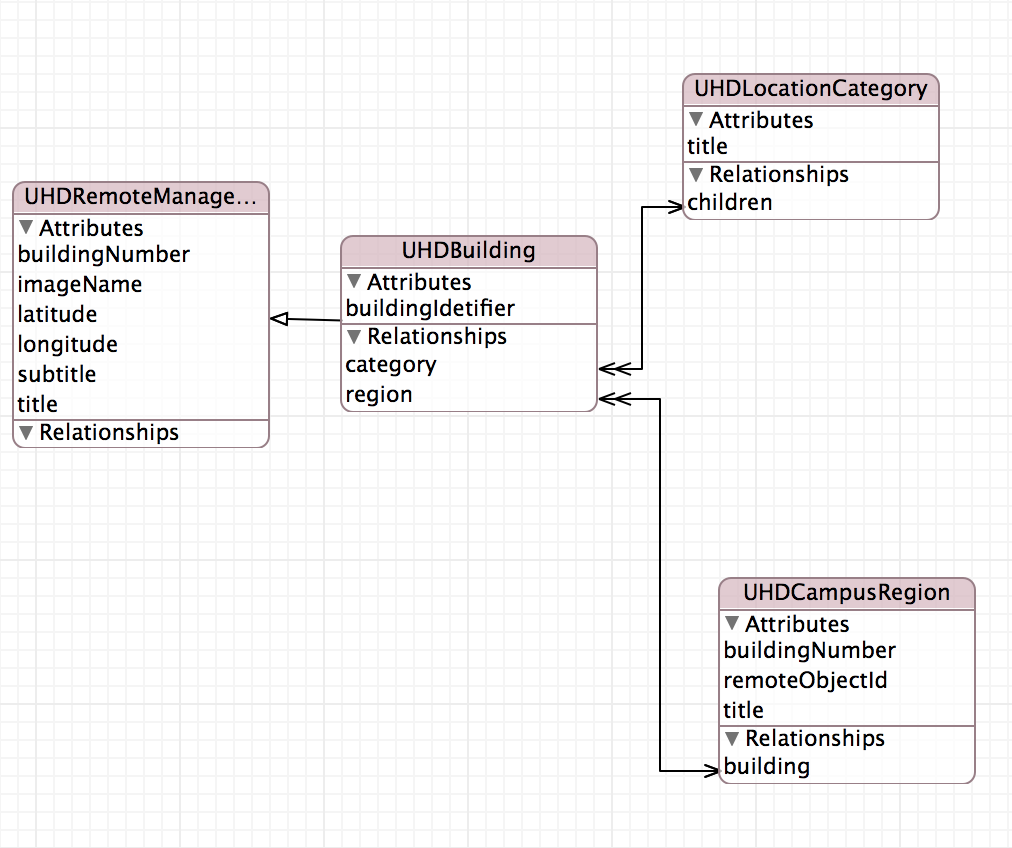
\includegraphics[scale=0.6]{DataModel.png}}
\caption{Data Model der Maps}
\end{figure}

Zunächst sollen die Gebäude in einer Klasse dargestellt werden. Dazu benötigt man eine \textsf{UHDRemoteManagedLocation} \textbf{GENAUER?!}. Diese ordnet jedem Gebäude verschiedene Eigenschaften, wie Ort oder Titel zu. Die Gebäude selbst werden in der Klasse \textsf{UHDBuilding} implementiert. Dazu wird jedem Objekt der Klasse ein \textsf{buildingIdentifier} übergeben, welcher den Titel richtig zusammensetzt. Dies liegt darin begründet, dass beispielsweise Gebäude im Neuenheimer Feld alle den Zusatz \emph{INF} tragen, sodass dem Gebäude nur eine \textsf{buildingNumber} zugeordnet werden muss. Der eigentliche \textsf{title} des Gebäudes setzt sich dann aus beiden Teilen zusammen, was aufgrund der überschriebenen Getter-Methode des \textsf{buildingIdentifier} geschieht. Um eine solche Charakterisierung der Gebäude zu erhalten, muss jedem Gebäude eine Region in Heidelberg zugeordnet werden. Dazu wird eine weitere Klasse \textsf{UHDCampusRegion} erstellt, die jedem Gebäude eine solche \textsf{region} zuorndet. Um weiterhin zwischen Gebäuden verschiedener Fakultäten oder auch Verwaltungsgebäuden zu unterscheiden, wird eine weitere Klasse \textsf{UHDLocationCategory} erstellt, die jedem Objekt der Klasse \textsf{UHDBuilding} eine \textsf{category} zuordnet.

\subsection{Implementierungsdateien}

\begin{objclst}

\end{objclst}


\section{Darstellung der verschiedenen Views}

Im \textsf{NavigationViewController} kann über den Button \textsf{Campus} die Anzeige der \textsf{MapView} erreicht werden. Dort gibt es zunächst die Option die Karte in verschiedenen Ansichten darzustellen. Es gibt die Wahl zwischen \textsf{Map}, was die Standardarstellung auf der Karte in iOS ist, \textsf{Satellite} oder \textsf{OVERLAY} \textbf{NACHTRAGEN}. In den ersten beiden Optionen werden die einzelnen Gebäude durch Stecknadeln dargestellt. Durch die Auswahl einer solchen Stecknadel erhält man zunächst grundlegende Informationen, wie den Titel, in einer Art Sprechblase angezeigt. Das Tappen auf diese Sprechblase öffnet ein neues Fenester, welches alle Informationen zum Gebäude anzeigt. Die dritte Kartendarstellung ist ein wenig aufwendiger zu implementieren, denn diese ist keine von Apple vorgefertigte Anzeigeoption. Stattdessen wurde dazu aus verschiedenen PDFs der Universität, welches die Gebäude mit Namen anzeigt, benutzt, um ein sogenanntes \emph{Overlay} zu erzeugen. Das heißt über die \textsf{MapView} wurde das PDF gelegt und dort die Koordinaten an bestimmten Fixpunkten eingetragen. Wir haben uns für diese zusätzliche Darstellung entschieden, da sie dem Benutzer einen viel besseren Überblick über die Gebäude der Universität liefert, als die eigentliche Karte in iOS. 


\section{Implementierung der View Controller}


\newpage
\chapter{Zusammenfassung}

\end{document}